\documentclass[11pt]{article}
% =========================================================================
% SHARED STYLE FILE for 11_Master_Projects reports
% Visual style follows 0_Thesis_Submission/24m0553_AK_Gaurav_Mtech_Report.pdf:
% serif body font, blue hyperlinked TOC/links, ruled section headings,
% IITB-style title page, formal academic report structure.
% =========================================================================

\usepackage[a4paper,margin=1in]{geometry}
\usepackage{xcolor}
\usepackage{graphicx}
\graphicspath{{../images/}}
\usepackage{amsmath,amssymb}
\usepackage{booktabs}
\usepackage{caption}
\usepackage{float}
\usepackage[hidelinks]{hyperref}
\usepackage{titlesec}
\usepackage{enumitem}
\usepackage{setspace}
\usepackage[T1]{fontenc}
\usepackage{lmodern}
\usepackage{microtype}

% Every \includegraphics call is automatically framed with a thin black
% border (matches the printed look of figures/photos/charts in the source
% reports). \oldincludegraphics is kept available for institutional
% logos/seals on title pages, which should remain unframed.
\let\oldincludegraphics\includegraphics
\setlength{\fboxsep}{1pt}
\setlength{\fboxrule}{0.6pt}
\renewcommand{\includegraphics}[2][]{\fbox{\oldincludegraphics[#1]{#2}}}

\definecolor{thesisblue}{RGB}{0,0,205}
\hypersetup{
  colorlinks=true,
  linkcolor=thesisblue,
  urlcolor=thesisblue,
  citecolor=thesisblue,
  filecolor=thesisblue
}

\onehalfspacing
\setlength{\parskip}{6pt}
\setlength{\parindent}{0pt}

\titleformat{\section}
  {\normalfont\Large\bfseries}{\thesection}{1em}{}
\titleformat{\subsection}
  {\normalfont\large\bfseries}{\thesubsection}{1em}{}
\titleformat{\subsubsection}
  {\normalfont\normalsize\bfseries}{\thesubsubsection}{1em}{}

\newcommand{\reportTitlePage}[7]{%
  % #1 = Report title
  % #2 = Course code & name (e.g. "CE 605: Applied Statistics")
  % #3 = Subtitle/topic line (e.g. "Project Report 2: Network Analysis")
  % #4 = Author block (can be multi-line with \\ for group projects)
  % #5 = Supervisor name(s)
  % #6 = Programme line (e.g. "M.Tech in Transportation Systems Engineering")
  % #7 = Month/Year
  \begin{titlepage}
    \centering
    \vspace*{0.5cm}
    {\large\bfseries #2}\par
    \vspace{0.3cm}
    {\Large\bfseries #3}\par
    \vspace{1.2cm}
    {\Huge\bfseries #1}\par
    \vspace{1.5cm}
    \oldincludegraphics[width=3.2cm]{../../assets/iitb_logo.png}\par
    \vspace{1.2cm}
    Submitted by:\par
    \vspace{0.2cm}
    {\bfseries #4}\par
    \vspace{0.8cm}
    Under the Supervision of\par
    \vspace{0.2cm}
    {\bfseries #5}\par
    \vspace{1.2cm}
    #6\par
    Department of Civil Engineering\par
    \textbf{Indian Institute of Technology Bombay}\par
    Mumbai -- 400076, India\par
    \vspace{0.3cm}
    #7\par
  \end{titlepage}
}

\newcommand{\reportAbstract}[1]{%
  \section*{Abstract}
  #1
  \vspace{0.5cm}
}


\title{Network-Theoretic Analysis of Spatial Rainfall Correlation Structures Across India}
\author{Abhijeet Kumar Gaurav}
\date{}

\begin{document}

\reportTitlePage
  {Network-Theoretic Analysis of Spatial Rainfall Correlation Structures Across India}
  {CE 605: Applied Statistics}
  {Project Report 2: Network Analysis}
  {Abhijeet Kumar Gaurav \\ Roll No.: 24M0553}
  {Prof.\ \href{https://www.civil.iitb.ac.in/faculty/details/prof-bellie-sivakumar}{Bellie Sivakumar}}
  {M.Tech in Transportation Systems Engineering}
  {Autumn 2024}

\pagenumbering{roman}

\reportAbstract{
Rainfall over India exhibits strong spatial correlation driven by shared climatic and geographic
influences, yet conventional station-by-station statistical analysis struggles to capture the
system-wide structure of these dependencies. This report applies complex network theory to
monthly rainfall records from 20 meteorological grid stations (drawn from a national archive of
over 4000 grids spanning January 1961 -- December 2014) to represent stations as nodes and their
pairwise rainfall correlations as edges. Adjacency structures are constructed at three correlation
thresholds (0.2, 0.3, and 0.5), and the resulting networks are characterised using degree centrality,
clustering coefficient, average shortest path length, global efficiency, and the harmonic mean of
shortest path lengths. Results show that low thresholds produce a densely connected, near-complete
network in which nearly all stations are reachable within a single hop, while progressively higher
thresholds isolate a smaller set of strongly correlated ``core'' stations and fragment the remainder
into sparser clusters. These findings illustrate how threshold selection governs the trade-off between
network-wide connectivity and the specificity of identified relationships, offering a scalable,
data-driven framework for studying regional rainfall dependence relevant to water-resource planning
and climate-risk assessment.

\vspace{0.3cm}
\noindent\textbf{Keywords:} Complex Network Theory; Rainfall Correlation; Degree Centrality;
Clustering Coefficient; Global Efficiency; Spatial Statistics
}

\newpage
\tableofcontents
\newpage
\pagenumbering{arabic}

\section{Introduction}
This project examines the spatial structure of monthly rainfall variability across India through
the lens of complex network theory. Rather than treating each meteorological station in isolation,
the analysis represents each station's rainfall record as a \emph{node} and quantifies the
statistical similarity between every pair of stations as a weighted or thresholded \emph{edge}.
This graph-based representation converts a purely statistical question, namely ``how correlated is
rainfall across space?'', into a structural one that can be probed with the well-established
toolkit of network science.

Framing rainfall data as a network is useful for several reasons:

\begin{enumerate}
  \item \textbf{Modelling interconnectedness.} Representing each grid as a node and each significant
  correlation as an edge makes it possible to visualise which regions move together and which remain
  comparatively isolated, revealing how weather patterns propagate spatially.
  \item \textbf{Identifying patterns and anomalies.} Metrics such as degree centrality and the
  clustering coefficient surface structure, for instance groups of stations sharing a climatic
  driver, that is difficult to see in a raw correlation table.
  \item \textbf{Assessing vulnerability and resilience.} Highly connected (high-centrality) stations
  represent critical nodes for regional water-resource management; understanding which stations play
  this role informs planning for droughts and floods.
  \item \textbf{Supporting real-time monitoring.} Because the network can, in principle, be updated as
  new data arrives, the same framework supports continuous tracking of how correlation structure
  evolves, which is valuable for early warning of shifts in rainfall distribution.
  \item \textbf{Feeding integrated climate models.} Quantified spatial dependence structures can be
  incorporated into broader climate models that combine rainfall with other variables such as
  temperature and humidity.
\end{enumerate}

The remainder of this report is organised as follows: Section~2 describes the study area and data;
Section~3 presents the network-theoretic methodology and the metrics used; Section~4 reports the
results across three correlation thresholds; Section~5 discusses the implications of threshold choice;
and Section~6 concludes.

\section{Study Area and Data Collection}

\subsection{Study Area}
The study area covers India, where monthly rainfall has been digitised for over \textbf{4,000
meteorological grids}. Each grid represents a specific geographic location and captures a localised
rainfall time series.

\subsection{Data Collection}
The parent dataset spans \textbf{54 years}, from \textbf{January 1961 to December 2014}, giving 648
monthly records per grid. For this project, a subset of \textbf{20 rainfall stations} was assigned,
allowing a focused, computationally tractable analysis while preserving the spatial diversity of the
national dataset.

\section{Methodology}
This analysis uses network theory to explore spatial relationships within rainfall data across
different regions of India. Network theory models real-world systems as a collection of nodes and
edges, enabling relationships, dependencies, and structural properties of the system to be captured
quantitatively.

\subsection{Network Theory Overview}
Each node in the constructed network represents a rainfall station (grid point), and each edge
indicates a statistically significant correlation between the rainfall records of two stations.
Strong correlations suggest similar rainfall behaviour, which may be driven by shared climatic
influences or geographic proximity. Figure~\ref{fig:illustrative} shows a simple illustrative network
with six nodes and eight links, of the same type constructed in this study at a larger scale.

\begin{figure}[H]
  \centering
  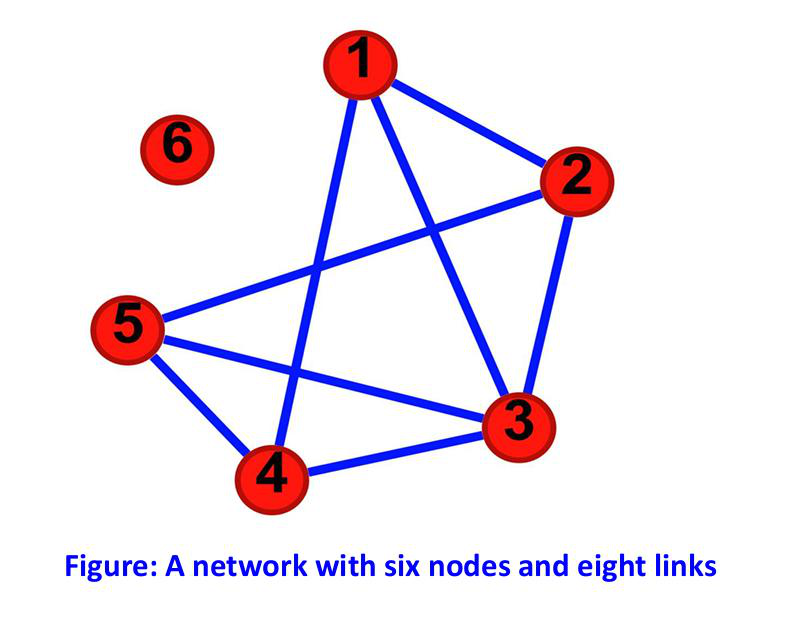
\includegraphics[width=0.45\textwidth]{fig_illustrative.png}
  \caption{Illustrative network diagram showing nodes and links.}
  \label{fig:illustrative}
\end{figure}

\subsection{Key Network Metrics}

\subsubsection{Degree Centrality (DC)}
Degree centrality measures the number of direct connections a node has with other nodes in the
network. In the rainfall network, it indicates how many other stations a given station is closely
related to, based on a chosen correlation threshold.
\[
DC = \frac{k}{N-1}
\]
where $k$ is the number of neighbours of node $i$ and $N$ is the total number of nodes in the network.
A higher degree centrality indicates that a station's rainfall pattern is shared with more locations
in the network.

\textbf{Procedure:} (i) compute the pairwise correlation between all station pairs; (ii) apply a
threshold (0.2, 0.3, or 0.5) to decide which correlations are considered significant; (iii) build the
binary adjacency matrix; (iv) count, for each node, the number of connections above the threshold and
apply the formula above.

\subsubsection{Clustering Coefficient (CC)}
The clustering coefficient quantifies the tendency of a node's neighbours to form connections among
themselves, i.e. to form local clusters. A higher clustering coefficient indicates that a station's
correlated neighbours are also correlated with each other, suggesting a localised region of similar
rainfall behaviour.
\[
c_i = \frac{2E_i}{k_i(k_i - 1)}
\]
where $E_i$ is the number of edges that actually exist among node $i$'s $k_i$ neighbours.

\subsubsection{Shortest Path Length}
The shortest path length between two nodes is the minimum number of edges that must be traversed to
connect them. In this context, it indicates how directly rainfall influence or similarity may
propagate from one station to another; shorter paths suggest closer correlation or regional
influence.

The \textbf{average shortest path length} $L$ measures the overall efficiency of the network in
terms of connectivity:
\[
L = \frac{1}{N(N-1)} \sum_{i \neq j} l_{ij}
\]
where $l_{ij}$ is the shortest path length between nodes $i$ and $j$. A smaller $L$ implies stations
are closely interconnected on average, while a larger $L$ suggests stations are relatively isolated
from one another in terms of rainfall similarity.

\subsubsection{Global Efficiency}
Global efficiency measures how efficiently influence can spread across the network by averaging the
\emph{reciprocal} of shortest path lengths over all node pairs:
\[
E_{glob} = \frac{1}{N(N-1)} \sum_{i \neq j} \frac{1}{l_{ij}}
\]
Higher global efficiency indicates that stations are well connected even across long (graph-distance)
separations, facilitating rapid transmission of climatic influence across the network.

\subsubsection{Harmonic Mean of Shortest Path Lengths}
The harmonic mean of shortest path lengths is a robust connectivity measure that reduces the influence
of outliers or disconnected node pairs: $HM = 1/E_{glob}$. Lower harmonic-mean values indicate that
nodes can generally reach one another more easily, suggesting a well-integrated network.

\subsection{Steps in Analysis}
The overall analysis pipeline proceeds through four stages: \textbf{data preparation}
$\rightarrow$ \textbf{network formation} $\rightarrow$ \textbf{computation of network metrics}
$\rightarrow$ \textbf{results visualisation}. Correlation thresholds of \textbf{0.2, 0.3, and 0.5}
were applied at the network-formation stage to study how connectivity structure changes as the
significance criterion is tightened.

\section{Results}
After preprocessing and cleaning, a refined dataset of valid monthly rainfall records from 20 grids
across India (January 1961 -- December 2014) was obtained, with each grid represented as a node in
the correlation network.

\subsection{Correlation Matrix and Network Formation}
Figure~\ref{fig:heatmap} shows the pairwise Pearson correlation coefficients between all 20 stations
as a heatmap, using a diverging (``coolwarm'') colour scale: warmer colours indicate positive
correlation and cooler colours indicate negative correlation. Diagonal cells are left blank, since a
station's self-correlation is trivially 1 and is not relevant to the inter-station analysis.

\begin{figure}[H]
  \centering
  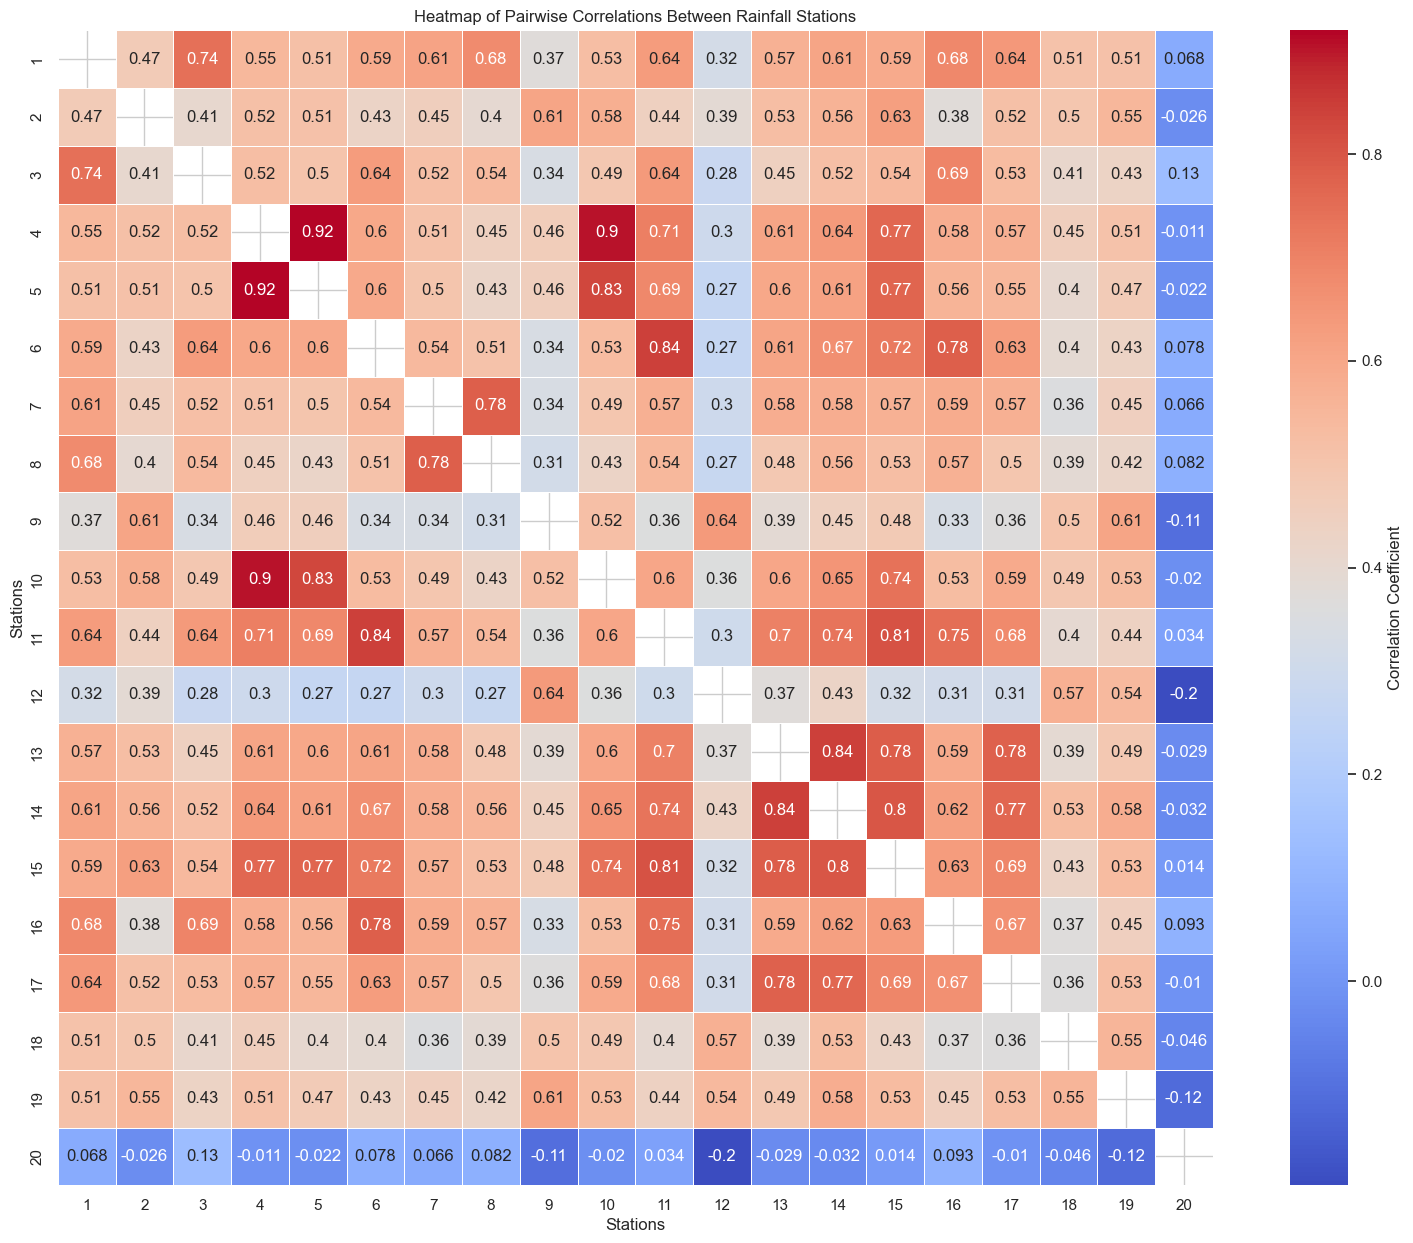
\includegraphics[width=0.9\textwidth]{fig_correlation_heatmap.png}
  \caption{Heatmap of pairwise correlations between the 20 rainfall stations.}
  \label{fig:heatmap}
\end{figure}

The adjacency matrix at each threshold is derived directly from this correlation matrix: an edge is
placed between two stations whenever their correlation coefficient exceeds the chosen threshold. As
expected, higher thresholds progressively remove weaker edges, isolating nodes that fail to meet the
stricter criterion, while lower thresholds retain a much denser set of connections.

\subsection{Global Efficiency and Harmonic Mean}
Table~\ref{tab:globaleff} summarises the global efficiency and harmonic mean of the network at each
threshold.

\begin{table}[H]
  \centering
  \caption{Global efficiency and harmonic mean across correlation thresholds.}
  \label{tab:globaleff}
  \begin{tabular}{@{}ccc@{}}
    \toprule
    \textbf{Threshold} & \textbf{Global Efficiency} & \textbf{Harmonic Mean} \\
    \midrule
    0.2 & 0.450000 & 2.222222 \\
    0.3 & 0.442105 & 2.261905 \\
    0.5 & 0.360965 & 2.770352 \\
    \bottomrule
  \end{tabular}
\end{table}

As the threshold increases, global efficiency decreases and the harmonic mean of shortest path
lengths increases, reflecting the network's progressive fragmentation as only the strongest
correlations are retained.

\subsection{Degree Centrality and Clustering Coefficient}
Table~\ref{tab:dcall} reports the degree centrality (DC) and clustering coefficient (CC) of each node
at thresholds 0.2, 0.3, and 0.5. At threshold 0.2, nodes 1--19 are near-fully connected (DC
$\approx 0.947$) and node 20 is isolated (DC~=~0), giving a network-average DC of 0.900; at threshold
0.3 the network-average DC is 0.868; and at threshold 0.5 it falls to 0.563.

\begin{table}[H]
  \centering
  \small
  \caption{Degree centrality (DC) and clustering coefficient (CC) by node across the three correlation thresholds.}
  \label{tab:dcall}
  \begin{tabular}{@{}c cc cc cc@{}}
    \toprule
    & \multicolumn{2}{c}{\textbf{Threshold 0.2}} & \multicolumn{2}{c}{\textbf{Threshold 0.3}} & \multicolumn{2}{c}{\textbf{Threshold 0.5}} \\
    \textbf{Node} & \textbf{DC} & \textbf{CC} & \textbf{DC} & \textbf{CC} & \textbf{DC} & \textbf{CC} \\
    \midrule
    1  & 0.947368 & 1.000000 & 0.947368 & 0.960784 & 0.789474 & 0.733333 \\
    2  & 0.947368 & 1.000000 & 0.947368 & 0.960784 & 0.473684 & 0.777778 \\
    3  & 0.947368 & 1.000000 & 0.894737 & 1.000000 & 0.578947 & 0.945455 \\
    4  & 0.947368 & 1.000000 & 0.894737 & 1.000000 & 0.736842 & 0.824176 \\
    5  & 0.947368 & 1.000000 & 0.894737 & 1.000000 & 0.684211 & 0.884615 \\
    6  & 0.947368 & 1.000000 & 0.894737 & 1.000000 & 0.684211 & 0.897436 \\
    7  & 0.947368 & 1.000000 & 0.894737 & 1.000000 & 0.631579 & 0.924242 \\
    8  & 0.947368 & 1.000000 & 0.894737 & 1.000000 & 0.421053 & 1.000000 \\
    9  & 0.947368 & 1.000000 & 0.947368 & 0.960784 & 0.263158 & 0.600000 \\
    10 & 0.947368 & 1.000000 & 0.947368 & 0.960784 & 0.684211 & 0.756410 \\
    11 & 0.947368 & 1.000000 & 0.947368 & 0.960784 & 0.684211 & 0.897436 \\
    12 & 0.947368 & 1.000000 & 0.631579 & 1.000000 & 0.157895 & 1.000000 \\
    13 & 0.947368 & 1.000000 & 0.947368 & 0.960784 & 0.631579 & 0.909091 \\
    14 & 0.947368 & 1.000000 & 0.947368 & 0.960784 & 0.842105 & 0.700000 \\
    15 & 0.947368 & 1.000000 & 0.947368 & 0.960784 & 0.789474 & 0.780952 \\
    16 & 0.947368 & 1.000000 & 0.947368 & 0.960784 & 0.684211 & 0.897436 \\
    17 & 0.947368 & 1.000000 & 0.947368 & 0.960784 & 0.736842 & 0.824176 \\
    18 & 0.947368 & 1.000000 & 0.947368 & 0.960784 & 0.263158 & 0.600000 \\
    19 & 0.947368 & 1.000000 & 0.947368 & 0.960784 & 0.526316 & 0.600000 \\
    20 & 0.000000 & 0.000000 & 0.000000 & 0.000000 & 0.000000 & 0.000000 \\
    \bottomrule
  \end{tabular}
\end{table}

At threshold 0.2, nearly every station shares a strong correlation with almost every other station,
so degree centrality is nearly uniform and clustering coefficients saturate at 1.0 (excluding the
isolated node 20). As the threshold is raised to 0.3 and then 0.5, degree centrality values spread out
considerably. Figure~\ref{fig:dcbar} compares degree centrality node-by-node across all three
thresholds, revealing a smaller set of consistently well-connected ``hub'' stations (e.g. nodes 1,
14, and 15 remain high at threshold 0.5) alongside stations that become comparatively peripheral.

\begin{figure}[H]
  \centering
  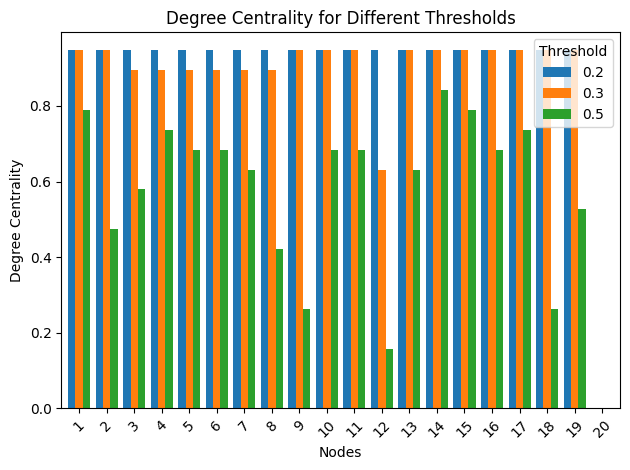
\includegraphics[width=0.75\textwidth]{fig_dc_barchart.png}
  \caption{Degree centrality by node across the three correlation thresholds.}
  \label{fig:dcbar}
\end{figure}

\subsection{Shortest Path Length and Network Visualisation}
Figures~\ref{fig:net02}--\ref{fig:net05} visualise the resulting networks at each threshold. At
threshold 0.2 the network is near-complete, with almost every pair of stations connected directly (a
shortest path length of 1). As the threshold rises to 0.3 and 0.5, edges are progressively pruned,
some shortest paths lengthen to 2 or 3 hops, and the network visibly sparsifies, with node 20
remaining disconnected across all thresholds.

\begin{figure}[H]
  \centering
  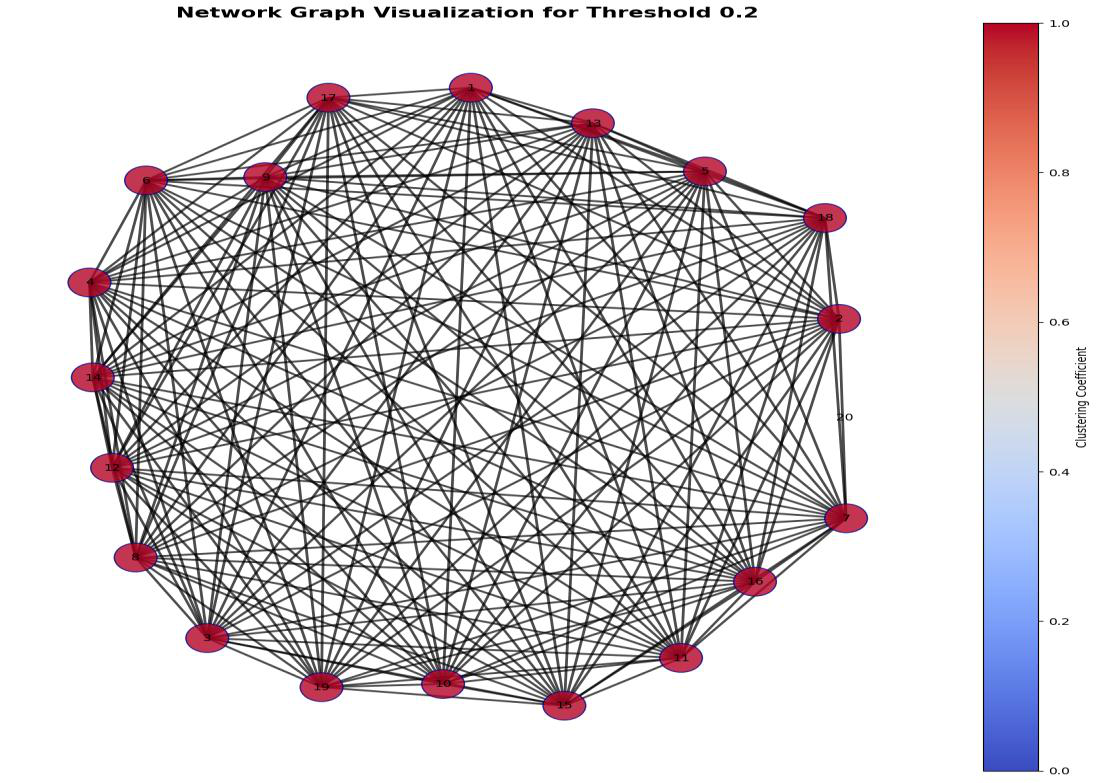
\includegraphics[width=0.7\textwidth]{fig_netgraph_t02.png}
  \caption{Network graph at threshold 0.2: a dense, near-complete graph.}
  \label{fig:net02}
\end{figure}

\begin{figure}[H]
  \centering
  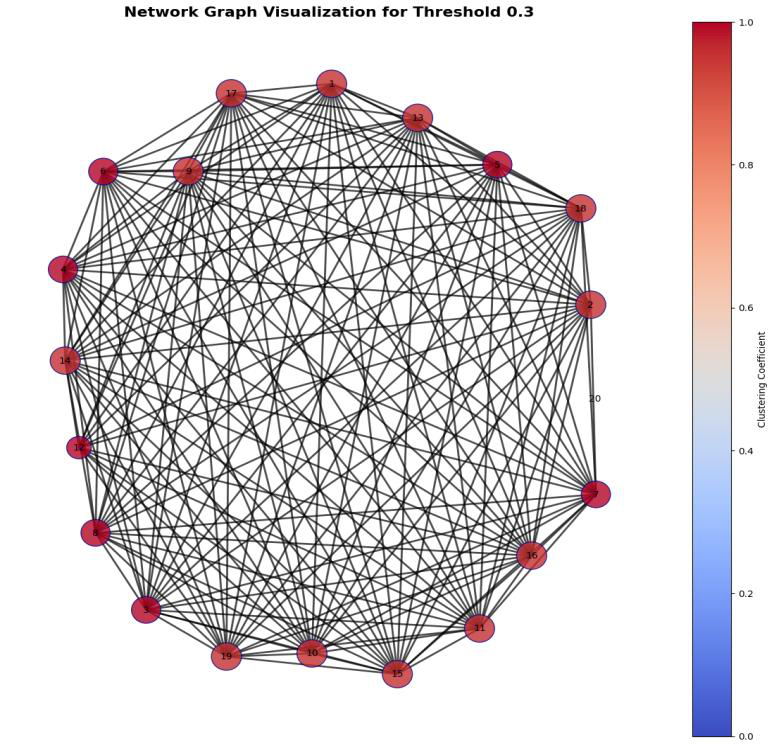
\includegraphics[width=0.7\textwidth]{fig_netgraph_t03.png}
  \caption{Network graph at threshold 0.3: moderately dense, with a small number of edges pruned.}
  \label{fig:net03}
\end{figure}

\begin{figure}[H]
  \centering
  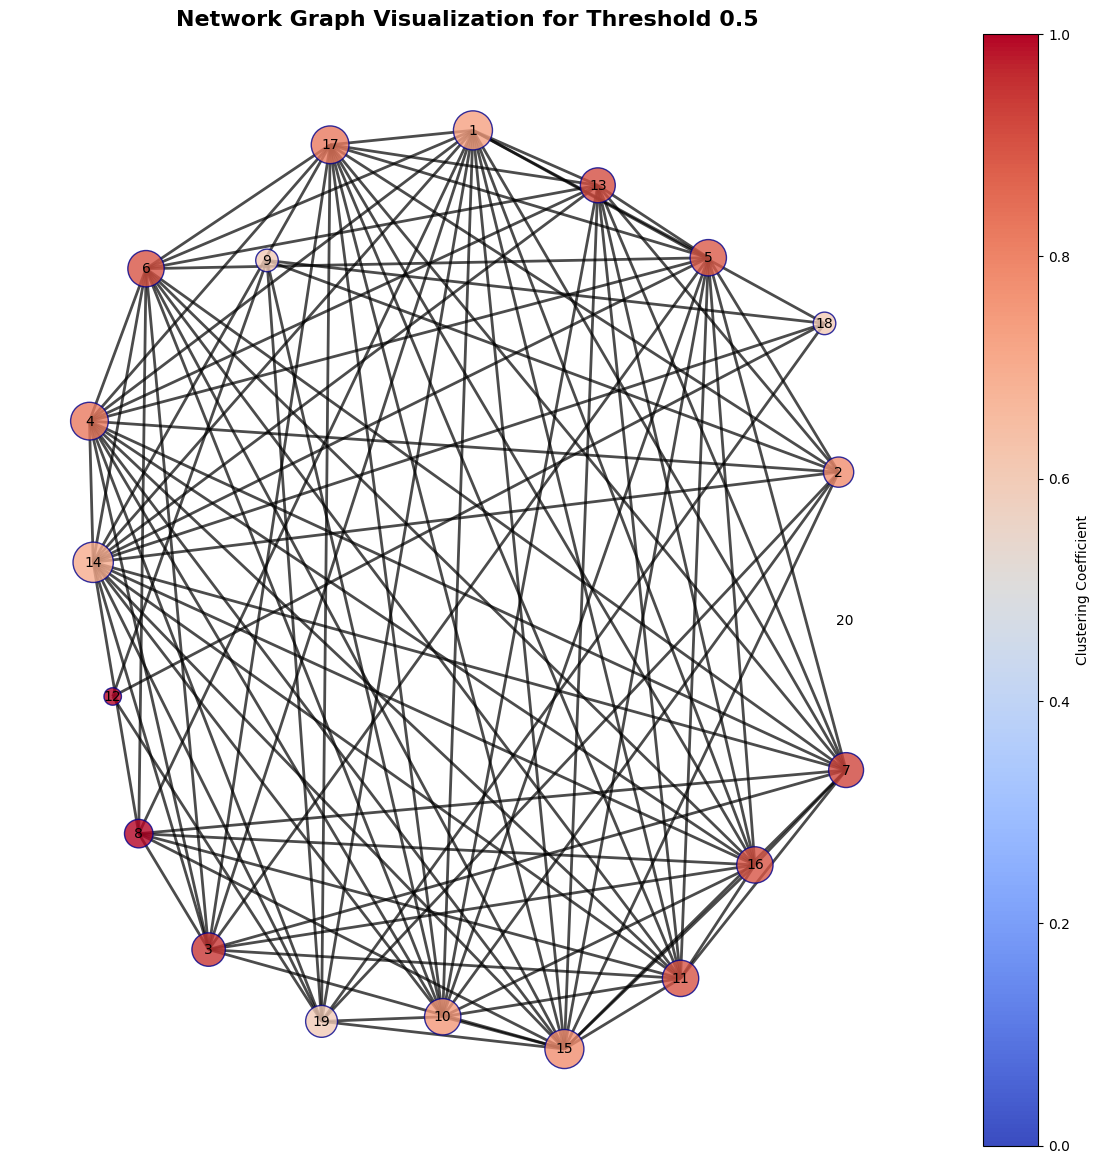
\includegraphics[width=0.7\textwidth]{fig_netgraph_t05.png}
  \caption{Network graph at threshold 0.5: a sparser, more selective network retaining only strongly
  correlated station pairs.}
  \label{fig:net05}
\end{figure}

\section{Discussion}

\textbf{Adjacency structure.} As the threshold value increases, the adjacency matrix shows
progressively decreased node connectivity. At threshold 0.2, nearly all stations are interconnected,
reflecting even weak correlations; at 0.3, some connections begin to drop, reducing network density;
at 0.5, only the strongest correlations remain, producing a sparser, more selective network. The
choice of threshold therefore materially impacts network structure: lower thresholds capture broad
interconnectivity, while higher thresholds focus on the most significant relationships, making the
network more robust and manageable for in-depth, targeted analysis.

\textbf{Global efficiency.} Global efficiency decreases as the threshold increases. At 0.2 the network
exhibits high global efficiency, meaning nodes can reach one another relatively quickly; at 0.5,
efficiency is reduced as fewer paths are available. Lower thresholds thus provide a more connected
network with better node accessibility, while higher thresholds, though reducing global efficiency,
may capture only the most reliable relationships, a balance that must be struck depending on the
analysis objective.

\textbf{Harmonic mean.} The harmonic mean of global efficiency is highest at threshold 0.2 and
decreases with increasing thresholds, reflecting the higher connectivity available at lower
thresholds and the resulting shorter, more direct paths between stations. High harmonic-mean values at
low thresholds indicate robust interconnectedness, valuable for analyses in which faster propagation
of influence across the network is important.

\textbf{Degree centrality.} Degree centrality decreases as thresholds increase. At 0.2, central nodes
have the highest degree centrality and serve as primary hubs; at 0.3 and 0.5, fewer nodes maintain high
centrality, emphasising only the most critical connections. This shows which nodes are most
influential within the network: lower thresholds highlight broad connections, while higher
thresholds reveal core nodes with significant, and presumably more climatically meaningful,
connections.

\textbf{Clustering coefficient.} The clustering coefficient is highest at lower thresholds,
particularly 0.2, indicating that local clusters of interconnected nodes are prevalent. As the
threshold increases, clustering decreases, showing more isolated nodes and fewer clusters. Higher
clustering coefficients at low thresholds suggest denser local groups, useful for analysing
community-based rainfall patterns; higher thresholds break these clusters apart, isolating key
regions.

\textbf{Shortest path length.} Shortest path lengths increase with higher thresholds. At 0.2, nodes
are generally close to each other, enabling rapid interaction across the network; at 0.5, the
network's average path length grows, with some nodes becoming more isolated or reachable only through
extended paths. Shorter paths at low thresholds indicate easy access and interconnectedness across the
network, while higher thresholds create distinct clusters reflecting regions with particular rainfall
patterns and more limited broader connectivity.

\subsection{Summary of Findings}

\begin{table}[H]
  \centering
  \small
  \caption{Summary of network metrics across correlation thresholds.}
  \label{tab:summary}
  \begin{tabular}{@{}p{2.3cm}p{2.3cm}p{2.3cm}p{2.3cm}p{4.0cm}@{}}
    \toprule
    \textbf{Metric} & \textbf{Threshold 0.2} & \textbf{Threshold 0.3} & \textbf{Threshold 0.5} & \textbf{Remark} \\
    \midrule
    Adjacency Matrix & High connectivity, dense network & Moderate connectivity, less dense & Sparse network, limited connections &
    Lower thresholds capture even weak correlations that may reflect broad seasonal or regional patterns; higher thresholds isolate closely linked stations likely sharing climatic or topographic drivers. \\
    \addlinespace
    Global Efficiency & High efficiency, easy reachability & Moderate efficiency & Low efficiency, selective paths &
    High efficiency at low thresholds implies rainfall patterns are interconnected across many stations; efficiency drops at high thresholds as only tightly correlated stations remain linked. \\
    \addlinespace
    Harmonic Mean & High, robust interconnectedness & Moderate & Low &
    Lower thresholds reveal a highly interconnected network where changes at one station may broadly impact others; higher thresholds filter out weaker connections. \\
    \addlinespace
    Degree Centrality & High centrality for several nodes & Moderate centrality & Few high-centrality nodes &
    Stations with high centrality at low thresholds act as rainfall-pattern hubs representing broad regional trends; only a few central stations remain connected at higher thresholds. \\
    \addlinespace
    Clustering Coefficient & High clustering, local clusters present & Moderate clustering & Low clustering, isolated groups &
    High clustering at low thresholds implies groups of stations with similar rainfall patterns, possibly reflecting shared microclimates; higher thresholds show more distinct, localised clusters. \\
    \addlinespace
    Shortest Path Length & Short paths, close accessibility & Moderate path lengths & Longer paths, limited accessibility &
    Shorter paths at low thresholds suggest many stations share similar rainfall trends; some stations become isolated at higher thresholds, representing distinct or unique rainfall regimes. \\
    \bottomrule
  \end{tabular}
\end{table}

\section{Conclusions}
Using varying correlation thresholds, this network analysis of 20 rainfall stations provides a
nuanced, structural view of rainfall correlation across regions of India. The network becomes
progressively more selective at intermediate and high thresholds (0.3 and 0.5), retaining only the
most strongly correlated stations and highlighting core groups with tightly coupled rainfall
patterns, likely driven by shared geographic or topographic factors such as proximity or similar
altitude. These clusters reflect microclimatic influences relevant to localised rainfall trend
studies, water-resource management, flood forecasting, and climate-adaptation planning.

The variation in global efficiency and harmonic mean across thresholds highlights the fundamental
trade-off between network-wide connectivity and specificity. Lower thresholds promote network-wide
efficiency and interconnectedness, useful for understanding broad, interconnected rainfall dynamics,
while higher thresholds reveal critical hubs and key stations with strong, direct correlations,
providing a focused view of specific, highly correlated rainfall patterns. This selective structure at
higher thresholds is valuable for identifying regions with distinct or isolated rainfall behaviour
that may be susceptible to unique climate risks.

Overall, this analysis underscores the importance of selecting an appropriate correlation threshold
based on the specific study objective: lower thresholds are preferable for capturing comprehensive
regional patterns, while higher thresholds enable focused, in-depth analysis of localised rainfall
phenomena. By applying network theory to rainfall data, this project demonstrates a scalable framework
for analysing spatial dependencies that can support climate research and inform regional water-policy
and planning decisions.

\begin{thebibliography}{9}
\bibitem{chen} Chen, G., Wang, X., \& Li, X. \textit{Fundamentals of Complex Networks: Models,
Structures and Dynamics}.
\bibitem{boccaletti} Boccaletti, S., Latora, V., Moreno, Y., Chavez, M., \& Hwang, D.~U. (2006).
Complex networks: Structure and dynamics. \textit{Physics Reports}, 424(4--5), 175--308.
\bibitem{newman} Newman, M.~E.~J. (2010). \textit{Networks: An Introduction}. Oxford University Press.
\bibitem{fang} Fang, K., Ma, J., Yang, J., \& Zhao, Q. (2015). Interannual variability and climate
controls on streamflow and flooding in China's paddy field areas. \textit{Journal of Hydrology}, 521,
275--286.
\bibitem{corpus} Graphical representation of genetic code algebra (2023).
\url{https://core.ac.uk/download/579840204.pdf}
\end{thebibliography}

\end{document}
